\chapter{Cognitive Operations: The Cognitive Toolbox} \label{chp:toolbox}
%reference that paper that shows the improvements in machine learning
\section{Overview}
As discussed in Section~\ref{ssec:intu},and illustrated in Figure~@TODOref the simplest imaginable description of sequential human cognition consists of a single step transforming the initial task information (along with background information) into an epistemic state that can be externally interpreted to choose a response. Assuming that this single operation $A$ transforms the initial knowledge base $x$ into final state $x'$ which is interpreted by external function $f()$, we can use the shorthand $f(x \longmapsto A)$, where $\longmapsto$ is a function that takes state point $x$ as input and produces a new state point $y$ as output, to summarise this process. 

To understand why this is poor choice of SCP, consider a general limitation of the SCP framework: we can only change the output of an SCP by changing the initial epistemic state, or by inserting/deleting a cognitive operation at an existing state point. Consider a case where the initial epistemic state is immutable. Thus, for $f(x \longmapsto A)$, the only possible changes are: $f(x \longmapsto \bar{B} \longmapsto A \longmapsto \bar{B})$, $f(x \longmapsto A \longmapsto \bar{B})$, $f(x \longmapsto \bar{B} \longmapsto A)$, $f(x \longmapsto \bar{B})$, and $f(x)$. Where $\bar{B}$ denotes the action of drawing some sequence of random, but valid cognitive state transitions. There is no way to change the operations that occur in $A$. Thus, even though Figure~@TODOref may be an appropriate model for the general reasoner of a given task, it imposes the explicit assumption that all other test subjects who achieved differing results, achieved only by completely ignoring the black-box process the general reasoners used, or else by inserting new operations only at the very start or end of the processing task. We will see an example in Section~@TODOref of cases where assumptions like that are simply not reflected by empirical data. 

Instead of using a single black-box operation to describe all cognition, it follows logically to use multiple smaller black box operations, each connected by a state point. Using this interpretation, cognitive operations for the general reasoner should be as extensive as possible, provided that they do not force implausible changes to describe deviant users or when used in other cognitive tasks. Figure~@TODOref captures this intuition as it applies to the Weak Completion Semantics. Indeed, as a non-monotonic logic that is already explicitly divided into discrete steps in the literature @TODOref, obvious candidate cognitive operations present themselves.

It is worth noting that this increased ability to model deviant reasoners comes at the cost of forcing more state points into the SCP being used.

The remainder of this section is devoted to expressing the exact properties, limitations, and concrete descriptions of cognitive operations.

@TODOlayout

\section{Cognitive Operation Space}
%then SCP space is cog op space size ^^ scp length
In principle, the number of cognitive operations available for use in an SCP is unlimited. We denote the space of all cognitive operations $\Omega$, and the space of all sequences $(A_0 \longmapsto ... \longmapsto A_n)$ with $\Omega^*$. There cannot and never will be an exhaustive search procedure to evaluate every possible way of manipulating an epistemic state (Proofs~\ref{proof:infiniteSCPs} and \ref{proof:infiniteSCPLength} illustrate the existence of valid SCPs for infinitely many different cognitive operations and valid SCPs of any length, respectively). However, there are ways of limiting the number of allowable cognitive operations. Lemma~\ref{lem:uniredundant} defines those cases in which there is redundancy in the set of all possible cognitive operations, Lemma~\ref{lem:taskredundant} focuses this concept on specific cognitive tasks which are to be modelled using SCPs.

\begin{proof} \label{proof:infiniteSCPs}
There are an infinite number of possible, valid SCPs, that can meet any goal condition $\gamma$ from input $x$ provided that at least one SCP exists that can reach goal condition $\gamma$ from input $x$.
\begin{enumerate}
\item There exist infinitely many cognitive operations $T \in \Omega$ which add a new variable from the set of all possible variable names $p \in P$.
\item There exist infinitely many cognitive operations $V \in \Omega$ which remove a variable from the set of all possible variable names  $p \in P$.
\item It follows that there exist infinitely many pairs $(T_i \in T, P_i \in P) \in W$ where $T_i$ adds a variable $p \in P$ to the resulting state point, and $V_i$ removes that variable from the resulting statepoint.
\item Then $f(x \longmapsto A) = f(x \longmapsto T_i \longmapsto V_i)$
\item Thus it follows that if $f(x \longmapsto A)\models \gamma$ then $f(x \longmapsto T_i \longmapsto V_i)\models \gamma$ for all $(T_i \in T, P_i \in P) \in W$.
\end{enumerate}
\end{proof}

\begin{proof} \label{proof:infiniteSCPLength}
If there exists an SCP which meets goal condition $\gamma$ of length $n$, then there exists an SCP that meets goal condition $\gamma$ of length $n+k$ where $k$ is any natural number.
\begin{itemize}

\item Proof~\ref{proof:infiniteSCPs} states that if $f(x \longmapsto A)\models \gamma$ then $f(x \longmapsto T_i \longmapsto V_i)\models \gamma$ for all $(T_i \in T, P_i \in P) \in W$.
\item Let $X$ be a partial SCP of the form $X=T_0 \longmapsto V_0 \longmapsto ... \longmapsto T_N \longmapsto V_{N}$ where $(V_i, T_i) \in W$
\item For odd lengths:
\begin{itemize}
\item  It follows that if $f(x \longmapsto A)\models \gamma$ then $f(x \longmapsto A \longmapsto \textrm{exp}(X))\models \gamma$, where $\textrm{exp}$ denotes the substitution of $X$ for its constituent parts.
\item Because $X$ always contains an even number of cognitive operations, then the length of the resulting SCP must be $n' = 1+v$ where $v$ is any even number.
\end{itemize}
\item For even lengths:
\begin{itemize}
\item Notice that $f(x \longmapsto A \longmapsto \textrm{exp}(X) \longmapsto X) \models \gamma$.
\item A appending $\longmapsto X$ to adds one to the length of any SCP.
\item Because we have shown that a suitable SCP of any odd length exists $n'>=n$, it follows that a suitable SCP of any even length $n'>n$ exists.
\end{itemize}
\end{itemize}

\end{proof}

\begin{lemma} \label{lem:uniredundant}
Given a cognitive operation sequence $A \in \Omega^*$, and external function $f()$, $A$ is redundant redundant iff one of the following holds:
\begin{itemize}
\item $(x \longmapsto B \longmapsto C) \models x'$ and $(x \longmapsto A) \models x'$ for every viable epistemic state $x$, $B \in \Omega^*$, $C \in \Omega^*$. 
\item $x \longmapsto A \models x$ for every viable epistemic state $x$.
\item $f(x \longmapsto B)=c$ for all $B \in \Omega^*$, where $c$ is a constant external decision.
\end{itemize}
\end{lemma}

\begin{lemma} \label{lem:taskredundant}
Given a limited set of cognitive operations $M=\{A_0, ..., A_n\}, A_x \in \Omega^*$, and external function $f()$, $A \in M^*$ is task redundant iff one of the following holds:
\begin{itemize}
\item $(x \longmapsto B \longmapsto C) \models x'$ and $(x \longmapsto A) \models x'$ for every viable epistemic state $x$, $B \in M^*$, $C \in M^*$. 
\item $x \longmapsto A \models x$ for every viable epistemic state $x$.
\item $f(x \longmapsto B)=c$ for all $B \in M^*$, where $c$ is a constant external decision.
\item There exists no epistemic state $x$ and sequences $B, C \in M^*$ such that $f(x \longmapsto B \longmapsto A \longmapsto C)$ is a valid SCP.
\end{itemize}
\end{lemma}

The total number of possible non-trivial SCPs of length $n$ for an SCP Task is given by $(|M|^L - R)$ where $|M|$ is the number of elements in the set of cognitive operations $M$, $L$ is the length of the SCP, and $R$ is the number of possible non-overlapping task redundant SCPs for the task. @TODOdefineOverlappingRedundantSCPs


\section{A Limited Set of Allowable Operations}
In practice it is impossible compute the set of all candidate SCPs when the set of allowable cognitive operations $M$ in a planning task is $\Omega^*$ or even $\Omega$. Without a length constraint Proof~\ref{proof:infiniteSCPLength} shows that it is not even possible to compute all possible SCPs for many SCP tasks with a finite set of allowable operations. Table~\ref{tbl:solutionSpace} summarises the properties of solution space under different SCP task conditions.

\begin{table}
\begin{center}

\begin{tabular}{ c c c c}
 \textbf{$M$} & \textbf{Finite Length Constraint} & \textbf{Finite Solution Space} & \textbf{Guaranteed Solution}\\ 
 $\Omega^*$ & None & \text{\sffamily X} & \checkmark \\ 
 $\Omega^*$ & Yes & \text{\sffamily X} & \checkmark \\ 
 $\Omega$ & None & \text{\sffamily X} & \checkmark \\ 
 $\Omega$ & Yes & \text{\sffamily X} & \checkmark \\  
 finite &  None & not guaranteed & \text{\sffamily X}\\  
 finite &  Yes &  \checkmark & \text{\sffamily X}
\end{tabular}
\caption{Solution space considerations of SCPs tasks as determined by length constraints and choice of cognitive operations.}
\label{tbl:solutionSpace}

\end{center}
\end{table}

\subsection{A Limited Set of Cognitive Operations}\label{ssec:limCogOp}
Readers should recognize that using the space of all possible cognitive operations for $M$ results in a computationally impossible task. No matter the other conditions imposed there will be infinitely many solutions to the given SCP task which satisfy $f()$.

But, beyond being just computationally infeasible, there are more empirical and philosophical objections to this approach. The first is that the human brain itself does not have infinite processing or space capabilities and so any model which allows for unrestricted data sizes in the set of allowable cognitive operations $M$ or in the number of resultant state points $M$ is not biologically well-founded\footnote{Because $\Omega$ is the set of all possible cogntive operations there must be at least one $m \in M$ such that, for any given input $x$, $x\longmapsto m$ results in a state point of size greater than the capacity of any storage system to hold.}. 

The second considerations is that there is considerable evidence in the literature that many problems can be modelled using logical frameworks which describe cognitive behaviour across a variety of tasks @TODOref. These frameworks reflect a more generally philosophy in cognitive psychology which is the idea of consistent cognitive motifs in reasoning. Using an infinite $M$ shows no discrimination at the time of task-formulation between those operations for which there is significant evidence and those which are fundamentally improbable.

\subsection{A Limited SCP Length}
As discussed in Section~\ref{ssec:limCogOp}, the human brain is constrained by a set of physical computational and storage limitation. In all case except those which are trivial or repetitive it would be computationally infeasible for the human mind to mimic an infinitely long SCPs. For this reason, SCPs of infinite length, though possible in a mathematical formulation, tend violate the spirit of the SCP Framework which is to \textit{accurately} model human cognition processes, not simply their conclusions.

It is worth noting that SCPs containing infinite loops can exist and can be evaluated at any time point $n$, they simply cannot be evaluated in their entirety.

\section{Purpose-Selected Cognitive Operations}
\subsection{Overview}
\subsection{Initialisation}
The initialisation cognitive operation (\texttt{init}) is always the first operation in an SCP. Thus, unlike every other cognitive operation, \texttt{init} has no prior cognitive operation from which to draw an epistemic state. Instead, it creates an epistemic state that reflects the initial inferential rules and variable assignments known by the agent. These rules and assignments are drawn from two distinct sources:
\begin{itemize}
\item \textbf{The initial interpretation of the task given}: in the case of the Suppression Task, for example, this rule corresponds to the given rules about Alice and the Library.
\item \textbf{Background information}: though this knowledge base is as large as every fact and inferential rule by known the participant, no computational is lost by only showing those facts and inferential rules that directly relate to the task in question\footnote{The question of precisely \textit{how} to sift through that enormous amount of information and select appropriate knowledge for the task at hand is an open problem.}.
\end{itemize}

In many ways it could be argued that the \texttt{init} operation is simply an aggregate cognitive operation that each encodes either a variable or rule insertion into the epistemic state (@TODOfig). The one caveat to this interpretation is that there must still be some first cognitive operation which takes no input and produces an epistemic state of suitable structure as output.

Because it is actually used as a shorthand for whatever sequence of sub-operations is needed to represent the initial epistemic state \texttt{init} is the only cognitive operation which differs on a task-by-task and a reasoner-by-reasoner basis. Every other cognitive operation is a uniquely-named pipeline whose internal structure is fixed for any task in which it appears.

\subsection{Variable Insertion}


\subsection{Variable Deletion}
\subsection{Variable Silencing}
\subsection{Variable Fixation}
\subsection{Adding Abnormalities}
\begin{figure} 
\begin{center}
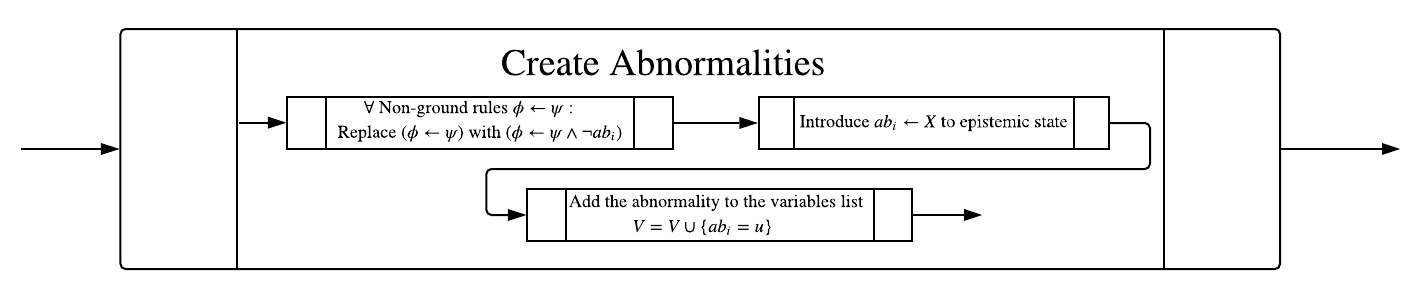
\includegraphics[width=\linewidth]{abnormalitySCP}
\end{center}
\caption{One possible formulation of a cognitive function to add abnormalities to variables. This formulation follows the intuition of Appendix~@TODOref.}
\label{fig:addAB}
\end{figure}

One of the most obvious candidates for a cognitive function that has evidence across a wide swathe of the cognitive literature (@TODOrefAFewPapers) is the idea of adding an abnormality variable to a problem that does not appear in the initial formulation of that problem. In Section~@TODOref and Section~@TODOref we discussed the idea of abnormalities as licenses for implication. The fact that we can point to several tasks in which an abnormality variable is added after formulation provides compelling evidence that creating these abnormality variables is a well-founded cognitive process that should be included in any comprehensive formulation of $M$. Figure~\ref{fig:addAB} shows one possible formulation of the \texttt{addAB} function for adding abnormalities to a knowledge base of the form $s=(KB,...)$ where $KB$ is a set of rules, and $V$ is a set of (variable name, variable value) pairs.



\subsection{Weakly Completing}
\begin{figure} 
\begin{center}
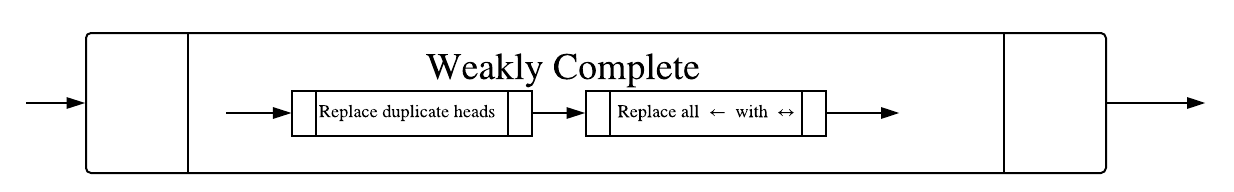
\includegraphics[width=\linewidth]{weaklycompleteSCP}
\end{center}
\caption{One possible formulation of a cognitive function to weakly complete a set of rules. This formulation follows the intuition of weak completion outlined in Section~@TODOsec.}
\label{fig:weaklycompleteSCP}
\end{figure}

Weak completion is an essential part of the WCS. Under the assumption that the WCS is a valid representation of human cognition in at least one scenario, any comprehensive set of cognitive operations $M$ must be able to mimic the Weak Completion of a knowledge base. Figure~\ref{fig:weaklycompleteSCP} how this can be achieved for any epistemic state of the form $s=(KB,...)$.

The 


\subsection{Semantic Operator}
\begin{figure} 
\begin{center}
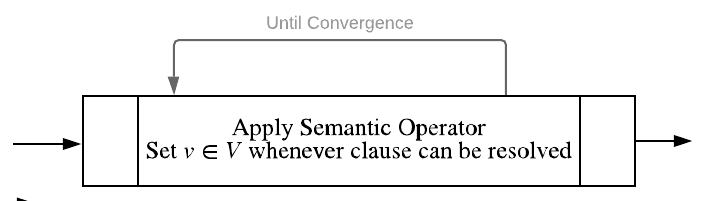
\includegraphics[width=\linewidth]{semanticOperatorSCP}
\end{center}
\caption{One possible formulation of a cognitive function to apply the semantic operator a congnitive state by temporarily setting all variables in $V$ to any value that can computed using the semantic rule in Equation~@TODOref. This process is repeated until $V$ is no longer updated. @TODOredoThisDigramToShowActualProcess}
\label{fig:semanticOperatorSCP}
\end{figure}

Another essential step in the WCS, the semantic operator is used to assign all variables to either True or False (explictly), or to Unknown (implicitly). Figure~\ref{fig:semanticOperatorSCP} illustrates one way in which this cognitive operation can be implemented for any epistemic state of the form $s=(KB,V,...)$.



\subsection{Default Inferencing}
If we assume that Reiter's default logic is a valid model of cognition for at least one task, it follows that an comprehensive formulation of $M$ must encode a cognitive operation for drawing inferences from a set of default rules. Figure~@TODOref illustrates the procedure for drawing such inferences from an epistemic state state of the form $s=(KB,V,D)$ where $KB$ is a set of inference rules, $V$ is mapping of variable names onto variable values, and $D$ is a set of default rules of the form $\frac{condition:exception}{conclusion}$ @TODOrewriteEquationWithStandardSymbols.

\section{Cognitive Operations as Aggregates}
%talk about combining existing cognitive operations for which there is strong evidence
An obvious and interesting idea follows from Proof~\ref{proof:aggregateValid} which is the idea of finding well-founded, uninterrupted epistemic operation sequences which are effective in modelling a variety of tasks and representing them as a single epistemic operation. We call this approach \textit{aggregating}, and it draws inspiration from recent advances in the field of reinforcement learning @TODORef in which simple tasks previously achieved are used as allowable actions when attempting to solve complex tasks.

This approach introduces the desirable property of shortening the total length of the SCP for a given set of cognitive tasks. However, it is evident from Proof~\ref{proof:aggregateExpressiveness} that any SCP task in which an aggregated subsequence of operations replaces those individual operations in $M$ may be less expressive than the same formulation in which the aggregated operations are still present.

\begin{proof} \label{proof:aggregateExpressiveness}
Given a cognitive task $\Pi=(x,f(), M, \gamma)$ in which $M=\{A_0,...,A_n\}$ and a second cognitive planing task $\Pi'=(x,f(),M')$ in which $M'= M \smallsetminus \{A_k,...,A_m\} \cup A'$, where $A'=(A_k \longmapsto... \longmapsto A_m)$ is a cognitive sequence containing some ordering of the other operations in $(\Pi \smallsetminus \Pi')$, $\Pi'$ is as expressive or less expressive than $\Pi$.

\item No more expressive:
\begin{itemize}
\item If $\pi' = (x\longmapsto A_p \longmapsto ... \longmapsto A' \longmapsto ... \longmapsto A_q)$ and $f(\pi)$ is a solution to $\Pi'$.
\item Let $\pi'' = (x\longmapsto A_p \longmapsto ... \longmapsto [A'] \longmapsto ... \longmapsto A_q)$.
\item Then $f(\pi'')$ is a solution to $\Pi'$ (Lemma~\ref{lemma:substitutionValid}).
\item $f(\pi'')$ is a valid solution to $\Pi$ because $\pi''$ uses only cognitive operations which occur in $\Pi$, $x$ is the initial epistemic state, and $f(\pi'') \models \gamma$. 
\end{itemize}

\item Less Expressive: Proof by counterexample
\begin{itemize}
\item If we assume that $\Pi'$ is strictly as expressive or more expressive than $\Pi$, then there exist no cases in which $\Pi'$ is less expressive.
\item Let $\gamma = \emptyset$, and $f(x)=True$ for all inputs (i.e. is trivially satisfied).
\item Let $x=\{\}$, $M=\{A_0,A_1\}$, $M'=\{A'\}$, $A'=\{A_0\longmapsto A_1\}$.
\item Then solutions of $\Pi$ are $f(x)$, $f(x \longmapsto A_0)$, $f(x \longmapsto A_1)$, $f(x \longmapsto A_0\longmapsto A_1)$ and $f(x \longmapsto A_1\longmapsto A_0)$.
\item Solutions of $\Pi'$ are $f(x), f(x \longmapsto A')$.
\item Thus, $\Pi'$ has fewer solutions that $\Pi$. A contradiction.
\end{itemize}
\end{proof}

@TODOexample?

The use of aggregates then, is a trade-off between sacrificing cross-reasoner accuracy and optimising a set of desirable heuristic properties such as length minimisation.

In many ways this compromise follows the philosophy of cognitive modelling in general. A neuron-by-neuron approach to predicting human behaviour (if one were ever possible) would give us extreme accuracy in modelling any human reasoner, but is too complex to be practical, and even if it were, would provide no abstracted information with which to find common motifs and inferences among reasoners. On the other extreme, modelling reasoners as (\textit{input}, \textit{output}) pairs perfectly captures the average predictions of a population, but proves very inaccurate for unseen individuals. State-of-the-art approaches to cognitive modelling like neural networks and non-monotonic logical frameworks seek generalizations which accurately capture the responses of most reasoners across as many tasks as possible by approximating human motifs in human reasoning and applying across multiple tasks and inputs.

The question of how to generate appropriate complex operation aggregates is a complex problem and is not discussed further in this thesis. It is, however a topic in which the author has significant interest.

\begin{proof} \label{proof:aggregateValid}
Given an SCP $\pi= f(x \longmapsto A_0 \longmapsto ... \longmapsto A_n)$, where $f(x)$ is an external evaluation function, $x$ is a state point, and $A_i \in \Omega$, any subsequence $A'=(A_k \longmapsto ... \longmapsto A_{k+l})$, $(k+l)<n$ of the cognitive operations in $\pi$ is a valid cognitive operation.
\begin{itemize}
\item Given that $\pi$ is a valid SCP, $x \longmapsto A_0$ must, by the definitions discussed in Section~@TODOref result in a valid state point.
\item It follows that $A'$ takes a valid state point as input, because $A_k$ took a valid state point as input.
\item It follows that $A'$ produces a valid state point as output, because $A_{k+1}$ produced a valid state point as output.
\item Therefore, $A'$ is a valid cognitive operation, by the definition in Section~@TODOref.
\end{itemize}
\end{proof}

\begin{lemma} \label{lemma:substitutionValid}
Let $\pi=(x\longmapsto A_0, ..., A', ..., longmapsto A_n)$ be a sequence of cognitive operations drawn from some cognitive task $\Pi=(x, \gamma, f(x), M)$ . And let $\pi'=(x\longmapsto [A_0], ..., A', ..., longmapsto A_n)$ where $[A]$ is the substitution of the aggregate operation $A'$ for $(A'[0]\longmapsto ... \longmapsto A'[t])$ . Then $f(\pi)=f(\pi')$.
\end{lemma}

\section{Epistemic State Structure Changes with Cognitive Operations}
%e.g. going to WCS to Default
The conception and mathematics of cognitive operations which produce output epistemic states points which differ in structure from the epistemic input structure are fairly straightforward.

Some cognitive operation $A$ with input base point structure $\textrm{struct}(s_k)$ and output base point structure $\textrm{struct}(s_{k+1})$ is called a \textit{structural transformation operation} iff $\textrm{struct}(s_k) \ne \textrm{struct}(s_{k+1})$.

The intuition behind structural state changes goes back to Albert Einstein's quote that opened this thesis ``Everything should be made as simple as possible, but no simpler.". In theory there is no restriction on SCP structure that would prevent every epistemic state passing an arbitrarily large number of variables and arguments. An SCP meant to represent a cognitive task where participant responses are consistent with propositional logic, for exmaple, could be accurately represented with an initial state $s_x=(KB)$ where $KB$ is simply the knowledge base of facts and rules given; but a researcher might equally use an epistemic state $s_y=(KB,V)$ where a variable $V$ is intended to store the values of each variable in $KB$; or even $s_z=(KB,V,D)$ where $D$ is a set of default rules. All three of these approaches would give an SCP the information required to evaluate the propositional task, but, if we know the task structure does not deal with uncertainty or show variation in reasoner responses, it becomes apparent that the set of default rules $D$ is unnecessary.

All of the possibilities given hold for the propositional task because $s_y$ and $s_z$ are both supersets of $s_x$ and $s_x$ is sufficient to model the task. Thus, provided the researchers do not believe that the task will make use of cognitive operations which require more complex state structures, $s_x$ is the simplest solution which meets the requirements of the researchers.

An obvious extension to the discussion above is the fact that a transformation from one state point structure to another when the input structure is a subset of the output structure is as easy as appending more structural variables to the input state. This transition hold in the example above in which a propositional logic compliant state point $s_x$ could be transformed into a WCS compliant state point $s_y$ or a default rule compliant state point $s_z$.

Unfortunately, structural change by appending variables are not universal obvious cases of structural transformation where they do not apply spring to mind. Such as the case where a more expressive state point must be changed to a less expressive state point structure. Imagine a case where a cognitive operation $B$ transforms a case point of $\textrm{struct}(s_z)$ to one of $\textrm{struct}(s_y)$. An intuitive example of this might be a hypothetical mental operation which handles biases in thinking. A student might begin at an epistemic state which believes ``usually, if I study for tests, I fail" and, through bias confirmation, come to believe ``If i study for tests, I fail", transitioning from a default rule, to immutable rule. 

In cases like this, it is up to the researcher to make several decisions: do I believe that the now empty set of variables $D$ no longer provides meaningful information? And how do I represent the change in the variables still present in the output state? These questions are very often task or function specific and cannot be answered in a general sense.

@TODOcompletestatetransformation

\section{Purpose-Built Cognitive Operations}
\subsection{Propositional Logic}
%no requirement of sequence, just exhaustive search
%not computationaly valid, NP-complete is too hard for human brain
An SCP for propositional logic must be able to take a set of rules and facts and draw the set of all valid inferences from that set using the standard propositional rules discussed in Section~@TODOref. To that purpose, we introduce a cognitive operation called \texttt{th} which draws all classically valid inferences from a set of logical rules\footnote{The reason that we do not introduce the functionality of the \texttt{th} cognition operation in the external evaluation function $f()$ is that doing so would make it impossible to directly use the derived theorems as part of another SCP.}.

\texttt{th} is by its nature a contrived cognitive operation and there is no expectation that it truly reflects human cognition. Instead, it serves as a benchmark operation with which to compare the results derived from knowledge base-driven logical approaches. Even a simpler congitive operation called \texttt{SAT} which determines if the given knowledge base it satisfiable still represents an \textit{NP-complete} (@TODOref) problem and is infeasible for any large knowledge base.

However, variations on the intuition of these two problems have real applications in cognitive modelling with SCPs and will be discussed throughout this section.

\subsection{Weak Completion Semantics}
\subsection{Default Logic}
\section{Two Approaches to Creating Cognitive Operations}
\section{Theoretical Approximation}
%must have empirical basis, but focused on reproducing mechanisms that have been proposed and substantiated in literature
%hand-curated
It seems reasonable that, given our desire to accurately model reasoning in participants, researchers creating cognitive functions for SCPs would choose to limit the set of allowable cognitive operations to those for which there is a sound theoretical basis. The reasons for this choice were discussed in Section~@TODOref.

The first approach to creating cognitive operations we will consider is the use of cognitive operations for which there is already evidence in our existing models of human cognition. This evidence can take a wide variety of forms: it may follow from our knowledge of physics (for example, the impossibility of storing a set of unrelated variables above a certain physical threshold); evolutionary biology (there cannot exist a class of organisms without some kind of reproductive drive); anatomy (there must exist cognitive processes that facilitate voluntary muscle activation); sociology (some neuronal connections seem to restrict the number of close friends a human can maintain @TODOref); or any other field of science. Using this information can allow researchers to predict what cognitive functions may play a role in observed empirical data. 

For the most part, theoretical approximation is a very powerful and well-justified mechanism for determining which cognitive operation could plausibly considered in the cognitive toolbox for a given task. Restricting the space of other cognitive operations which may play a part is also enabled by all the scientific fields mentioned above, complexity theory tells us that humans are unlikely to apply exhaustive classical logic reasoning to a task when the set of variables and rules to be considered is large because of physical limitations related to solving \textit{NP-complete} or harder tasks efficiently.

At present, the foundation of non-monotonic reasoning in cognitive modelling is this theoretical mindset, a well-founded explanation is found by borrowing from a relevent field (often psychology) and then tested against empirical evidence and across multiple cognitive tasks to show evidence that is a reasonable approximation of a mechanism in human cognition.


\section{Empirical Appoximation}
%finding cognitive operations using machine learning
%done by using search techniques to create and explore comparison space
Contrasting theoretical approximation is the field of constrained empirical approximation. Techniques ranging from neural networks and Markov models genetical inspired techniques consistently outperform humans in a huge variety of fields. Drawing on enormous databases of empirical data, modern artificial intelligence researchers have come to view machine learning as the most plausible way to create the first real thinking machine @TODOref.

@TODOfinish
